\begin{surferPage}{Cuártica de Kummer}
    En 1875, Eduard Kummer (1810 - 1893) fue la primer persona que planteó el 
    problema de hallar la cantidad máxima de singularidades $\mu(d)$ que podría tener una 
    superficie de grado $d$, y resolvió el caso de las cuárticas (d=4), para el cual
    halló que $\mu(4)=16$.

    A continuación, estudió más en detalle las cuárticas que tienen $16$ puntos singulares.
    En particular, construyó la hermosa familia: 
    \[\bigl(x^2+y^2+z^2-\gamma^2\bigr)^2 - \lambda
    \,y_0\,y_1\,y_2\,y_3,\]
    donde $\gamma$ es un parámetro libre y
    $\lambda = \frac{3\gamma^2-1}{3-\gamma^2}$. Los\\
     {\small
    $y_0=1-z-\sqrt{2}x$, \  
    $y_1=1-z+\sqrt{2}x$, \ 
    $y_2=1+z+\sqrt{2}y$, \ 
    $y_3=1+z-\sqrt{2}y$} \\
  son las caras de un tetraedro regular, para lograr una superficie simétrica.
  No todos los miembros de esta familia tienen $16$ singularidades, pero la mayoría sí.
  
  \begin{center}
    \vspace*{-0.2cm}\hspace*{-0.2cm}
    \begin{tabular}{@{}c@{\,}c@{\,}c@{\,}c@{\,}c@{}}
      \begin{tabular}{@{}c@{}}
        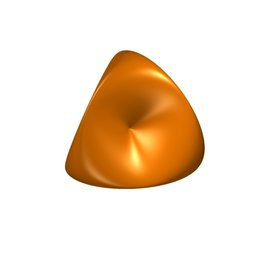
\includegraphics[height=1.4cm]{../../common/images/kummer_0}
      \end{tabular}
      &
      \begin{tabular}{@{}c@{}}
        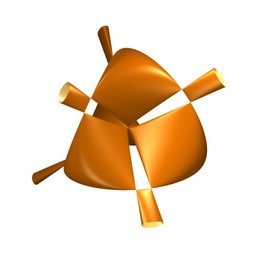
\includegraphics[height=1.4cm]{../../common/images/kummer_1}
      \end{tabular}
      &
      \begin{tabular}{@{}c@{}}
        
\includegraphics[height=1.4cm]{../../common/images/kummer_2}
      \end{tabular}
      &
      \begin{tabular}{@{}c@{}}
        
\includegraphics[height=1.4cm]{../../common/images/kummer_3}
      \end{tabular}
    \end{tabular}
  \end{center}
  \vspace{-0.2cm}  
   Esto es porque para algunos valores particulares de los parámetros, muchos puntos singulares
   pueden coincidir.
\end{surferPage}
